\chapter{Dynamical Systems Theory}\label{ch_dst}
\chapterauthor{Jeff Yoshimi, Scott Hotton}

  In chapters \extref{ch_act_functions}, \extref{ch_linear_algebra}, and \extref{ch_supervised} we have noted that when the ``play''  button 
\includegraphics[scale=.5]{./images/Play.png} is pressed in Simbrain  a dynamical process is simulated; neurons start firing and changing, weights will sometimes change their size, etc. Dynamical systems theory provides a formal, mathematical way to analyze these processes. A \emph{dynamical system} is a rule that says how a system changes its state in time. There is a clear visual way to understand dynamical systems: in terms of orbits in a state space (see Figs. \ref{F:stateSpaceParts}, \ref{F:hopfieldStateSpace}, \ref{F:pendulumStateSpace}, \ref{F:chaoticStateSpace}, and \ref{F:attractorsRepellers} below), trajectories that describe how a system behaves relative to different initial conditions. Pictures of these orbits provide a concrete way of understanding how a system  behaves, and can reveal information that would otherwise be hidden from us. Neural networks are dynamical systems,  which say how patterns of node activations, weight strengths, and other quantities change in time. When you press play in Simbrain, you run a dynamical system. Simbrain has special features, like the projection plot, which allow you to watch orbits unfolding in real time as a network runs.
% One value of dynamical systems theory is that it allows us to visualize a system. You can bypass the equations and get an initial feel for how it works, via the images.

% Use dog-beer pic for recurrent networks here? (See unsupervised chapter)
Dynamical systems theory is useful across all the domains of neural network theory. In connectionist models,  memories can be thought of as stable states or attractors in a recurrent network (that is, states which the system tends to go to over time), which can be visualized as points in an activation space. Pattern completion---e.g. seeing part of a picture and then imagining the missing part---can be understood as an initial state of a system settling in to an attractor. Learning can be understood as a dynamical process on the weight space of a network. More generally, connectionist theorists have thought of cognition as unfolding in a high-dimensional activation space, and learning as unfolding in an even higher-dimensional weight space. In computational neuroscience low level models of individual neurons are dynamical systems models, which describe how levels of calcium, sodium, spike rate adaptation, and other more abstract quantities change in time (in these models the Simbrain color only displays one of as many as 5 or more dynamically changing variables). In machine learning, recurrent networks are trained to reproduce dynamical sequences of data, and can generalize from existing data to new data: this kind of network can be trained to generate paintings in the style of a particular painter, or speech in the style of a particular speaker. There is also a body of theoretical work showing that neural networks can approximate any continuous dynamical system with arbitrary precision \cite{hornik1989multilayer}. This shows that the human brain has a great deal of flexibility in the kinds of behaviors and processes it could in principle produce. 
% Citations
% Smolensky. Occurrent vs. passive knowledge. Schemata

\section{Dynamical Systems Theory}

 In this section we consider the basic concepts of dynamical systems theory, and see 
how they can be used to study neural networks. 

% Image below the point shown is not above the line. Simple fix.
\begin{figure}[h]
\centering
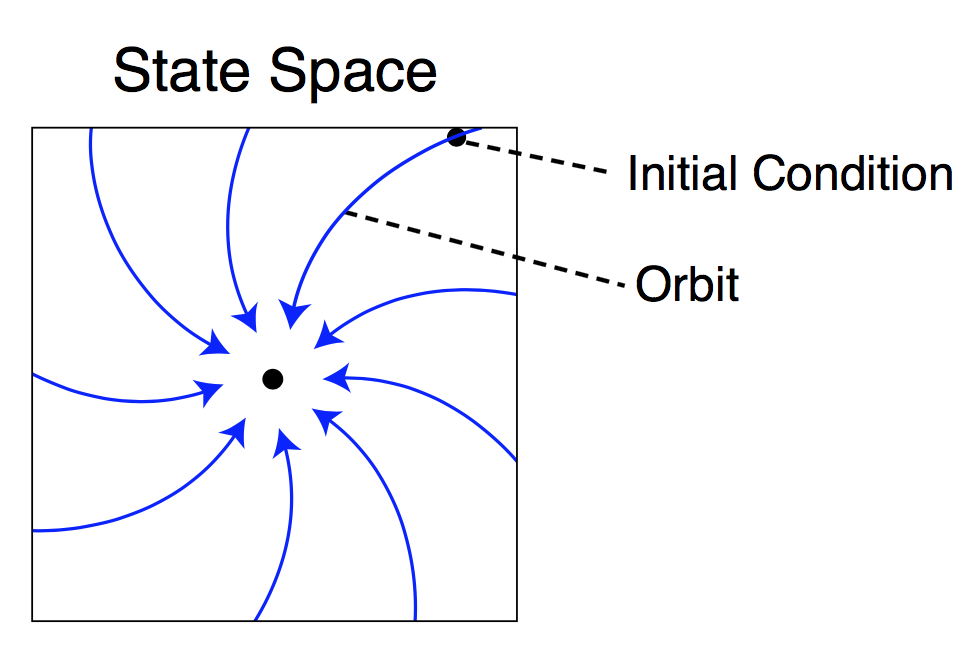
\includegraphics[scale=.45]{./images/StateSpaceParts.png}
\caption[Pamela Payne.]{Some basic components of a dynamical system. The square region is the \emph{state space} for a 2-dimensional system. Each point in that region is a \emph{state}. Each state can be treated as an \emph{initial condition}. When the system is run, an \emph{orbit} unfolds from the initial condition. A picture like this that shows selected orbits in the state space is a \emph{phase portrait}. The phase portrait shows in a concise, visually intuitive way what the dynamics of a system are. In this case we have a system with a single attracting fixed point. All orbits lead to that same state. Recurrent neural networks often display attractor dynamics.}
\label{F:stateSpaceParts}
\end{figure}

 We begin with the concept of a 
state. The word ``state'' is a general term to describe the condition of a
system. For instance a bar of iron can be in a magnetic state or nonmagnetic
state. The water in a jar can be in a frozen state but after being heated the 
water can change to a liquid state. A molecule can be in its ground state 
until it absorbs light whereupon it enters an excited state. People can be in
various emotional states. Oftentimes, states vary in a continuous way: the temperature
of a pot of water, the sound level of a plucked guitar string, and the firing rate of a neuron all move up and down as internal and external conditions change. Note that the same object can have lots of states, depending on what we are interested in. A human has a temperature, a height, and a weight, and all of these are changing. Any of them can be the focus of a dynamical systems analysis.
% State variable could be vector valued. 
% Redo with state vectors

Mathematically, the state of a system is represented by values for a collection of  state variables. Each \glossary{state variable} describes a numerical value associated with a system at a time. If we have variables describing the temperature and pressure of a pot of water, then the state of that system at a given time is the value of those variables at that time. If we have three variables describing height, weight, and temperature of a person, then a state of that person at a time is the value of those three variables at that time. If we have a neural network with $1000$ neurons, then we have $1000$ state variables, one for each neuron in the network. But again, it's up to us what we consider a state of the network to be. We might just focus on a few of those nodes. Or we might shift attention from nodes to the weights. We could consider the full matrix of $1,000,000$ weights in that network, which correspond to a million state variables. Or we could consider the combined set of activations and weight strengths, which would involve $1,001,000$ state variables.

A \glossary{state} of a system is a specification of values for all of the state variables which describe that system. If we model water using temperature (Farenheit) and volume (Liters) as our state variables,  a state for the pot of water might be $(89.8, 2)$. If we model a person using height (inches), weight (pounds), and blood sugar (mg/dl) as our state variables, a  state for the person might be $(60,150,75)$. A state for the nodes or the weights of the network is a large vector or matrix that is too long to write out here. Dynamics then describe how these states--e.g. activation vectors, weight matrices, or others collections of state variables--change in time.

The state of the network in Fig. \ref{F:hopfieldStateSpace} is $(-.8,.8)$, which are the values of two state variables $a_1$ and $a_2$, corresponding to the activations of the two nodes. However, recall that what we take to be a ``state'' of a system is up to us. So instead of looking at node activations, we could have looked at weight strengths. Then the state variables are $w_{1,1},w_{1,2}$ and the current state is  $(-1,-1)$. 

% The basin picture is misleading because the circle is not around a basin of attraction
\begin{figure}[h]
\centering
\raisebox{-0.5\height}{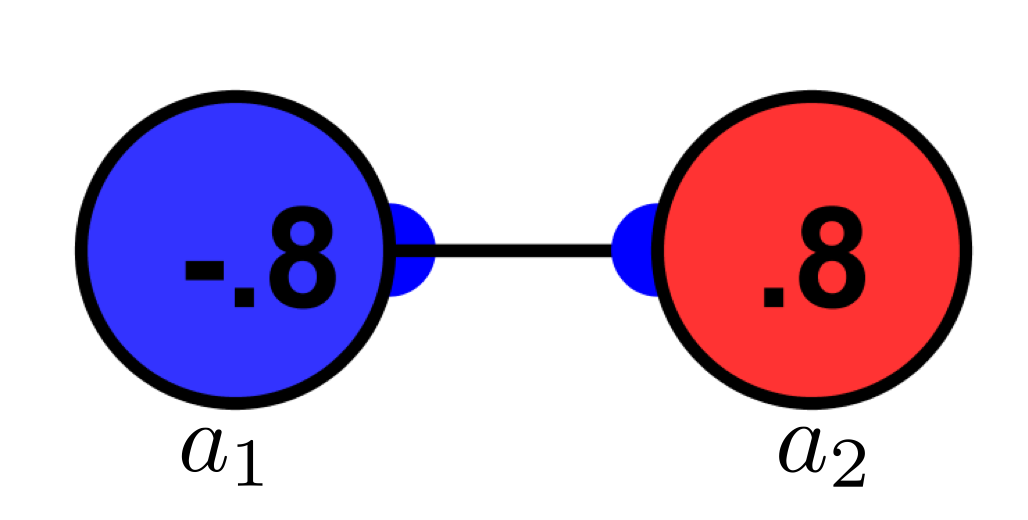
\includegraphics[scale=.2]{./images/HopfieldNetAttractor.png}}
\hspace*{1in}
\raisebox{-0.5\height}{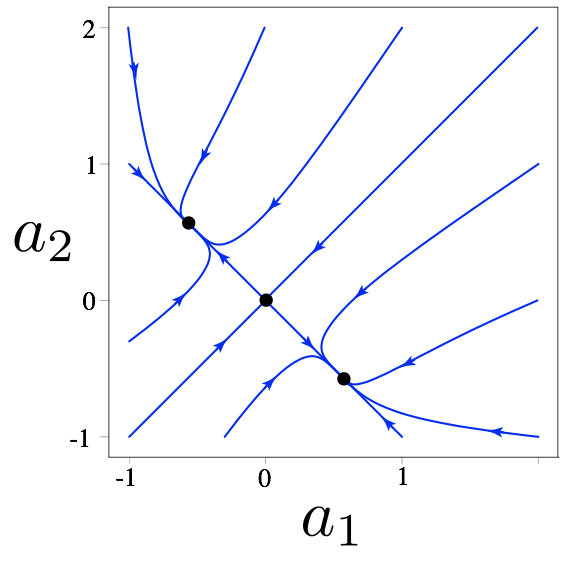
\includegraphics[scale=.6]{./images/HopfieldPortrait.png}}
\caption[Left: Simbrain screenshot; Right: Jeff Yoshimi.]{A 2 node recurrent network (left) and its phase portrait (right). The phase portrait has two fixed point attractors at $(-.8,.8)$ and $(.8,-.8)$, each with its own basin of attraction. There is a fixed point at the origin $(0,0)$ which is attracting in one direction but repelling in the other (a ``saddle-node''). This is a Hopfield network that was trained using a variant of the Hebb rule. The network stores two memories, corresponding to the two attractors. Cuing a memory can be interpreted as starting the network in an initial state. Recalling a memory from that cue can be interpreted as running the dynamics of the network and observing the initial state evolve towards one or the other attractor. By adding more nodes the network can encode more memories.}
\label{F:hopfieldStateSpace}
\end{figure}

  Having specified what a state of a system is we can consider its  \glossary{state space}, which is the set of  {\em all  possible} states of the system. For a neural network's activations, this means all possible activation vectors for that  network, all possible patterns of activity that could occur over all of its  nodes. So here the state space of a network is a subset of its \emph{activation space}. If we focus on a neural network's weights, the state space of a network is a subset of its \emph{weight space}. A network with $n$-nodes has an $n$-dimensional activation space and a weight space that can be up to $n^2$-dimensional (there are $n^2$ possible weights in a network of $n$ nodes; to see this recall that each weight can be represented as an entry in a matrix with $n$ rows and $n$ columns). Again, it is up to us to decide which features of a system to treat as state variables, and thus what to treat as a network's state space. In a neural network simulation, the state space  might be part of an activation space, a weight space, a combined activation / weight space, or perhaps something else.

The dynamics of a network unfold in its state space. In a neural network, this is often a high dimensional space, e.g. the 20-dimensional space of a network with 20 neurons. Recall from chapter \extref{ch_linear_algebra} that we can use dimensionality reduction techniques---like the projection plot in Simbrain---to visualize these dynamics in 2 or 3 dimensions.

% Add more figure refs below?
 An \glossary{initial condition} (or initial state) of a dynamical system is just the state the system begins in. For the case of a neural network's activation space, this is an initial 
specification of values for its  nodes. Theoretically any point in the state 
space can be taken as an initial condition although sometimes it may be 
difficult or impossible to actually start a physical system in some particular state (e.g. setting the position and velocity of the earth or setting a person's age). In Figs.
\ref{F:stateSpaceParts} and \ref{F:hopfieldStateSpace} any of the points shown could be taken as initial conditions. Each point corresponds to one pattern of  activation over the nodes of the corresponding network. Often we just randomly choose initial conditions.
In Simbrain we do this for activation states by selecting all the nodes of a network and then 
pressing the random button. If we repeatedly press the random button we end up 
putting the network in a whole bunch of different initial conditions, which is a useful way to explore the different ways the network can behave.

% The rule can be made more intuitive
We are now in a position to give a definition of a dynamical system:
\begin{quote}
\glossary{Dynamical system}: A rule that associates initial states of a system with (usually) future states of the system.
\end{quote}
(We say ``usually'' because the system can also associate initial states with themselves at the present time, and can sometimes also associate initial states with past states; these are called ``invertible'' systems).
A dynamical system can be thought of as a recipe for saying, given any initial 
point in state space (any initial condition), what states will {\em follow in 
time} for that system. If we know a system begins in state $(1,-1)$, the 
dynamical system will tell us exactly what states it will be in 4, 5, and 6 
seconds (or iterations) from now. And we can do this no matter what initial 
condition we place our system in. Thus dynamical systems are \emph{deterministic}, in
theory they allow us to completely predict the future of a system based on its 
present state. A major question in philosophy is whether the universe is deterministic, and thus describable by a dynamical system.\footnote{This is sometimes described in terms of ``Laplace's Demon.''   As Laplace himself said:  ``We ought to regard the present state of the universe as the effect of its antecedent state and as the cause of the state that is to follow. An intelligence knowing all the forces acting in nature at a given instant, as well as the momentary positions of all things in the universe, would be able to comprehend in one single formula the motions of the largest bodies as well as the lightest atoms in the world, provided that its intellect were sufficiently powerful to subject all data to analysis; to it nothing would be uncertain, the future as well as the past would be present to its eyes. The perfection that the human mind has been able to give to astronomy affords but a feeble outline of such an intelligence. (Laplace 1820)''. From Carl Hoefer's encyclopedia article: \url{https://plato.stanford.edu/entries/determinism-causal/}.}

\begin{figure}[h]
\centering
\raisebox{-0.5\height}{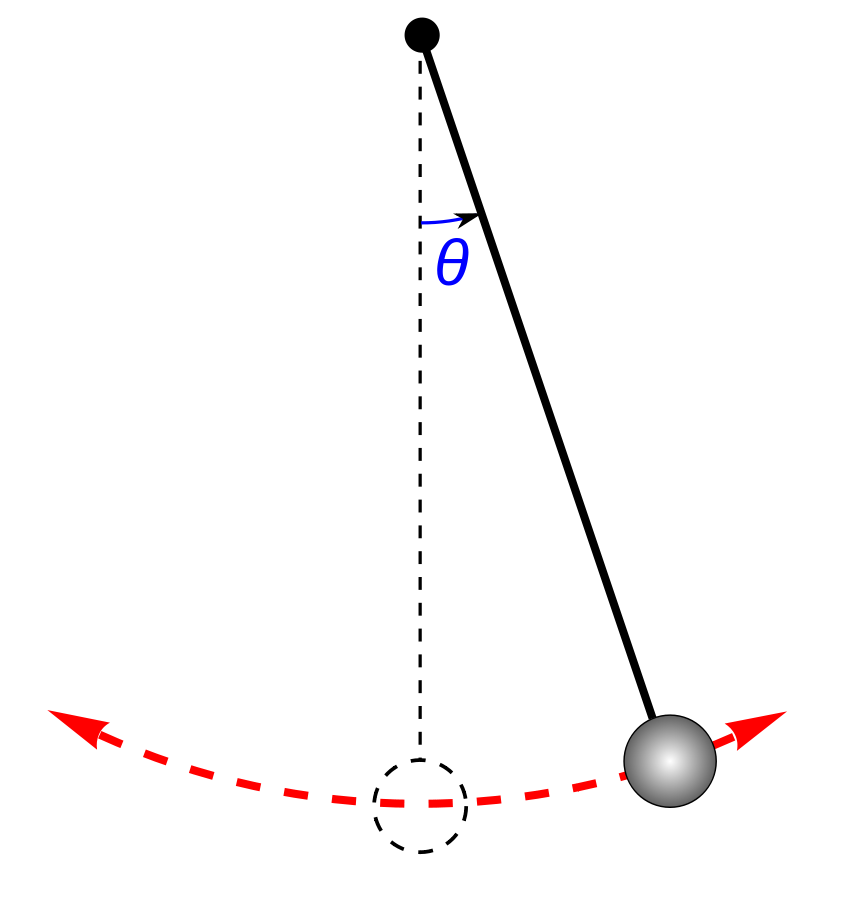
\includegraphics[scale=.15]{./images/Pendulum.png}}
\hspace*{.8in}
\raisebox{-0.5\height}{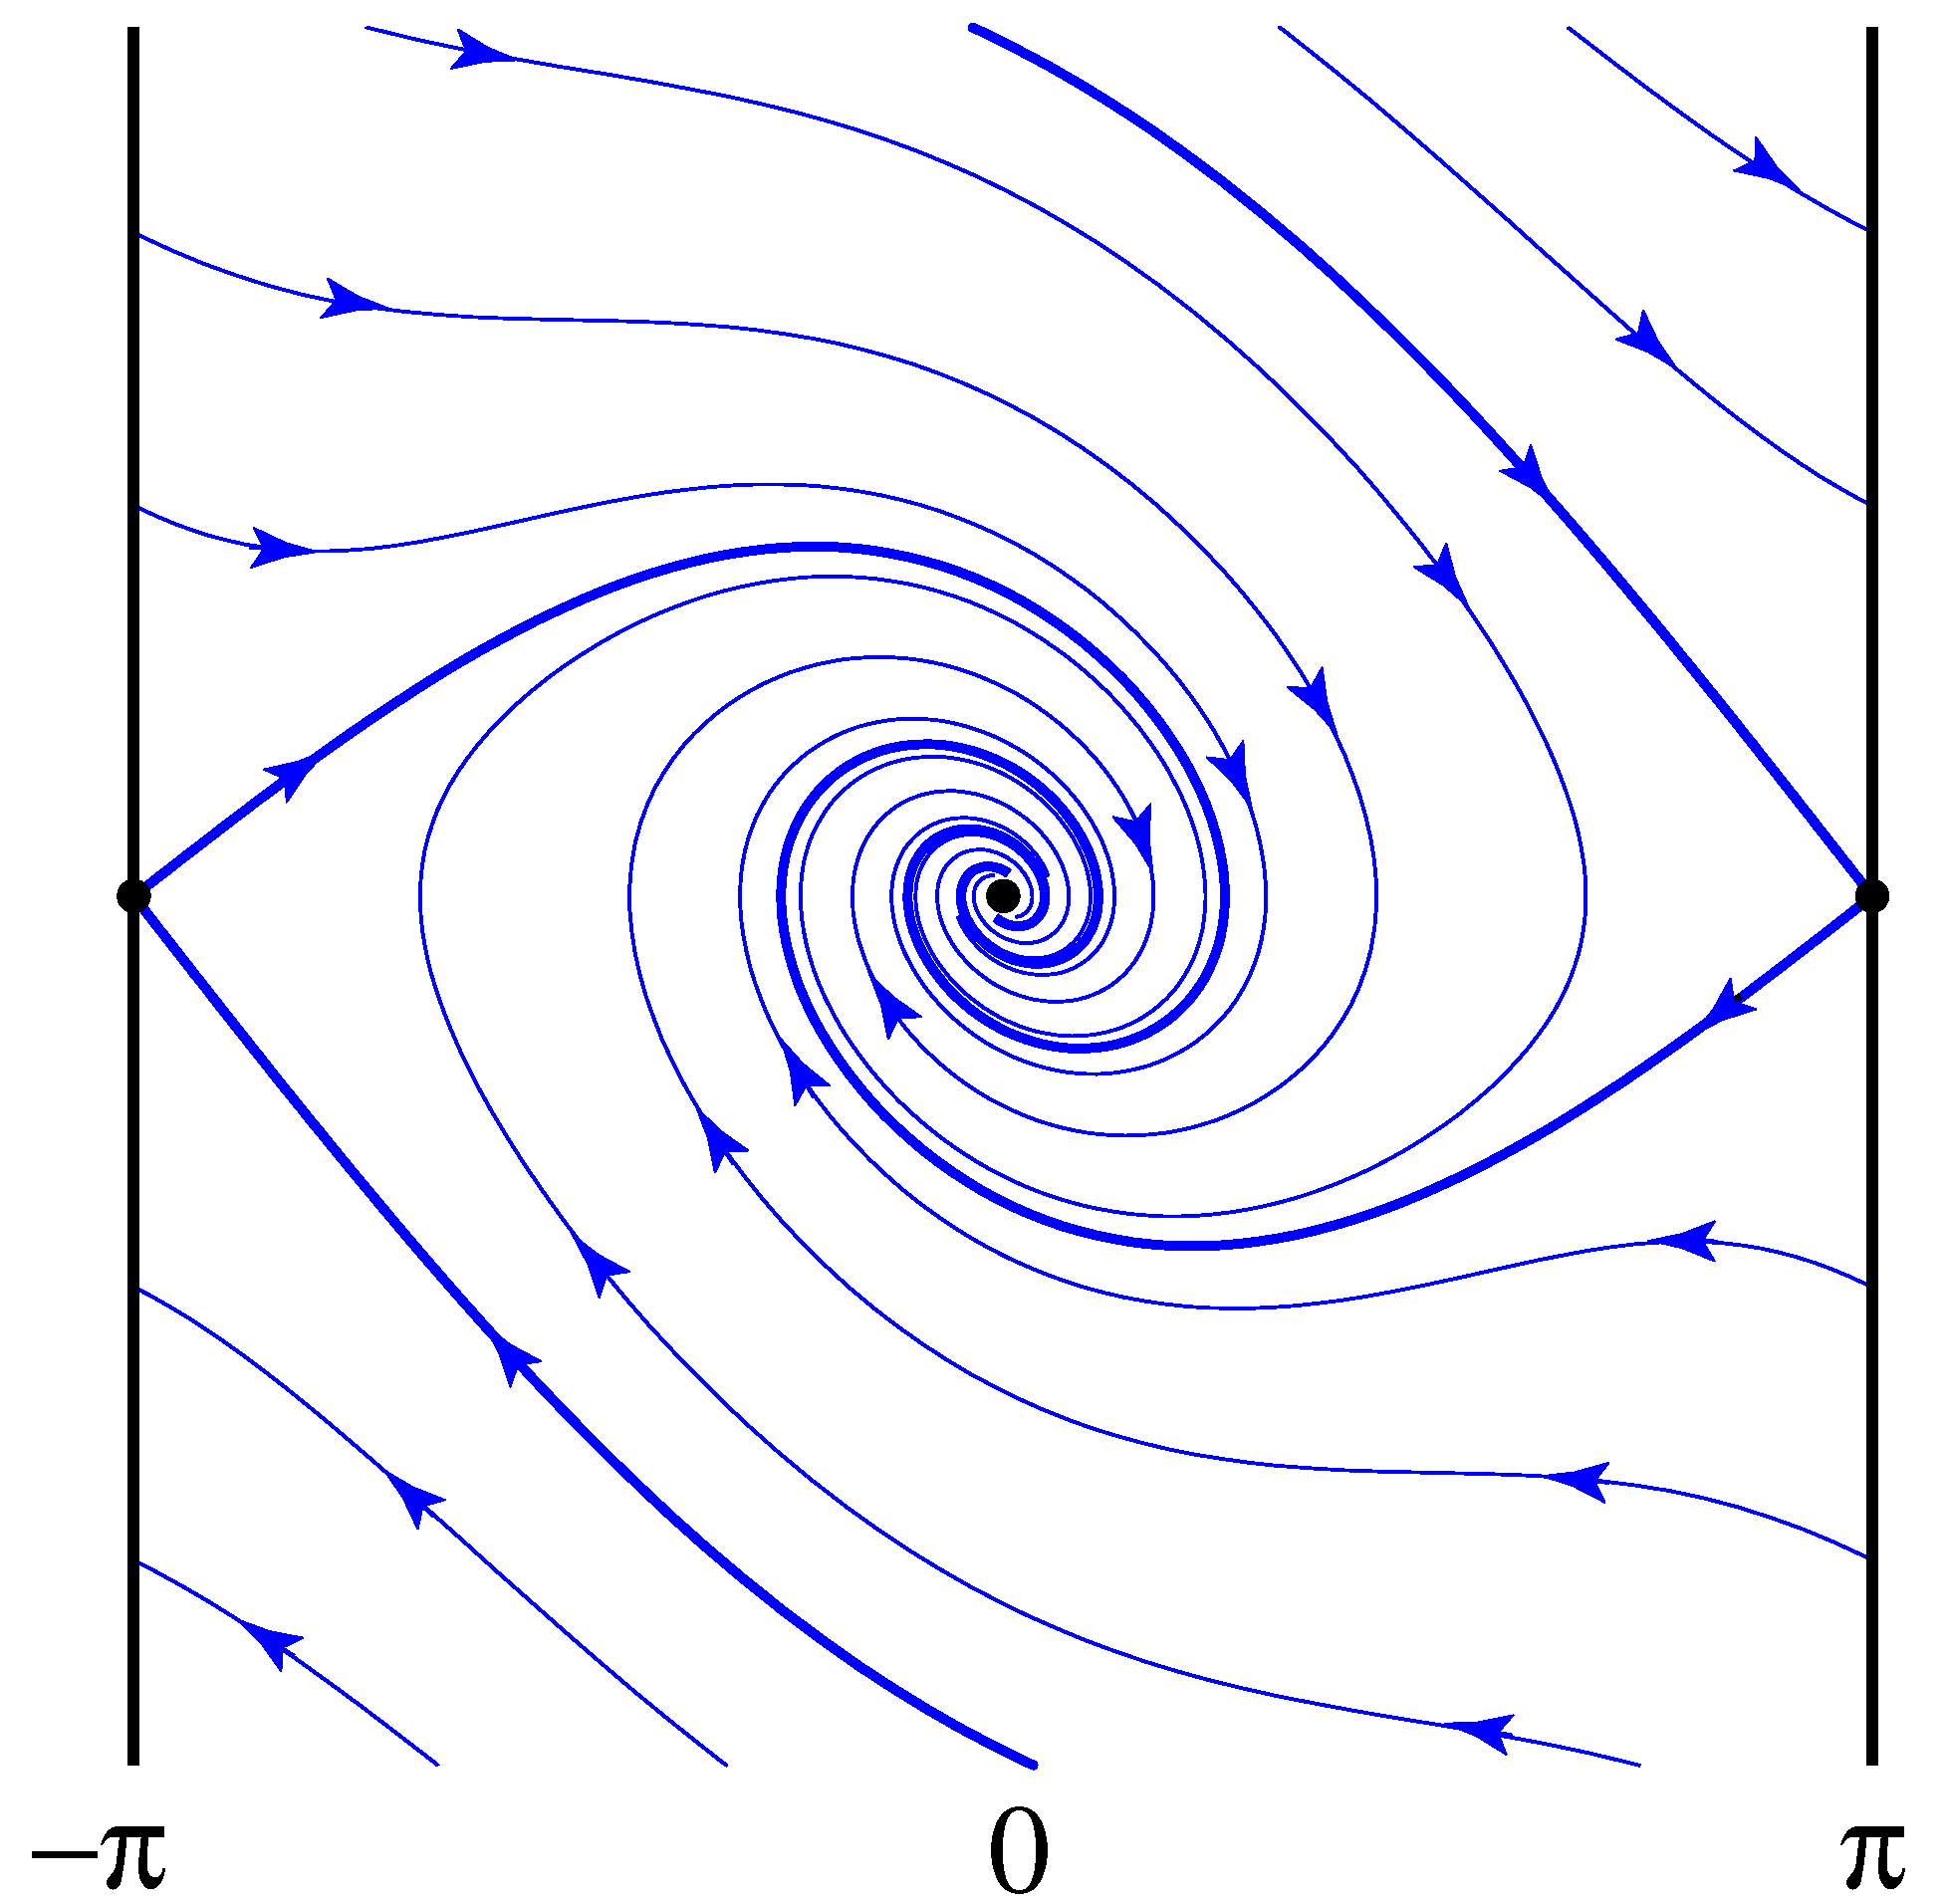
\includegraphics[scale=.2]{./images/PendulumPortrait.png}}
\caption[Left: From \url{https://commons.wikimedia.org/wiki/File:Simple_gravity_pendulum.svg}; Right: Scott Hotton.]{Penduluum (Left) and its state space with a phase
portrait (Right).}
\label{F:pendulumStateSpace}
\end{figure}

% Relate to recurrent relations? But if so note confusion that it seems it must recur
The mathematical category of dynamical systems is very abstract, and encompasses many more specific ideas in mathematics. For example, most differential equations count as dynamical systems, because they can be used to predict future states of a system from its current state. An iterated function is another kind of dynamical system (think of entering $2 \times 2$ on a calculator and repeatedly clicking the $=$ button).\footnote{In a differential equation time unfolds in a continuous way, while in an iterated function it unfolds in a discrete way. Thus we can distinguish continuous-time and discrete-time dynamical systems. Both types of system are modeled in neural networks and in Simbrain, e.g. a Naka-Rushton neuron is a continuous-time model, while a linear neuron is a discrete-time model. However, even the continuous time models actually run in discrete time in the underlying computer implementation.}
% Formal definition  in footnote. See text from braitenberg book

A pendulum is a classical example of a dynamical system. Pendulums have been studied extensively ever since Leonardo da Vinci designed fairly accurate clocks based on them. The state of a pendulum is given by two variables, one variable $\theta$ for the angular displacement of the pendulum from verticality and another variable $\dot{\theta}$ for the angular speed.\footnote{Note the dot over $\dot{\theta}$, which indicates the first derivative of $\theta$, i.e. rate of change of angular displacement, which is angular speed.}  If we start a pendulum with some chosen values for these two variables we can, at least in principle, say exactly how it will move forever in the future. Fig. \ref{F:pendulumStateSpace} shows a pendulum on the left and its state space on the right. The horizontal axis shows the angular displacement, $\theta$, and the vertical axis shows the rate of change of the angular velocity, $\dot{\theta}$. We can put the bob of the pendulum in any initial position and give it a push with any initial speed and the future of the pendulum will be determined. This behavior can be predicted by choosing the corresponding point in the phase portrait and following the orbit though that point. Eventually, because of friction, the orbit will close in on the point $(0,0)$ which corresponds to the pendulum hanging straight down without moving.\footnote{The state space is actually an infinitely long cylinder. Imagine wrapping the left and right edges of the state space in Fig. \ref{F:pendulumStateSpace} around and gluing them together.}

Neural networks are also like this. If we start a neural network off in some particular state--for example, if we specify values for all its nodes--then based on its 
update rules and the way it is wired together we can say just how it will behave for 
all future time. Thus, ``running'' a neural network, in Simbrain by pressing 
the step or the play button, corresponds to applying the dynamical rule that 
describes it. A neural network which is predictable in this way is a dynamical 
system. 

Can you think of ways to make a neural network {\em not} be a dynamical 
system?  One way is to add some random noise to a node. When you do that, it 
is no longer possible to predict with complete accuracy what future states will follow from the present state.

Since dynamical systems are deterministic, they can be used to predict exactly what future states will follow from any initial condition. However, \glossary{chaotic dynamical system} is a dynamical system whose future behaviors are difficult to predict. A chaotic system is still a dynamical system, so it's fully deterministic, but it's hard to predict how it will behave, especially moving farther in to the future. It's a kind of paradox: a chaotic system is fully determined by a set of equations, but it behaves in an erratic way.\footnote{The formal definition of chaos is a difficult and unresolved topic. One way to define chaos is in terms of ``sensitive dependence on initial conditions.'' In this view, a chaotic system is such that initial conditions that are extremely close to each other in the state space, can end up being very far apart given enough time. This is sommtimes called the \emph{butterfly effect}. Since weather is a chaotic phenomenon a small change in one part of the world, like the flapping of a butterfly's wings, can have a huge effect further in time. So for example, if you sneeze now (vs. not sneezing) it could influence food prices in Brazil a few months later.} To see chaos in Simbrain you can create a logistic activity generator. By default this rule produces chaotic dynamics (open its help page for more information). Many natural processes, like the weather, are thought to be chaotic. An example of chaotic behavior is shown in Fig. \ref{F:chaoticStateSpace}. Notice that given an initial condition it would be hard to predict where precisely that system would be at future times, even if we do know it would stay in that region of state space.
% https://en.wikipedia.org/wiki/Chaos_theory#/media/File:Chaos_Sensitive_Dependence.svg

% Possibly use this to show how they do different things; https://upload.wikimedia.org/wikipedia/commons/4/44/TwoLorenzOrbits.jpg
%Change color to blue
\begin{figure}[h]
\centering
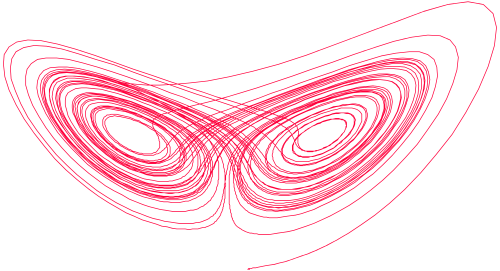
\includegraphics[width=0.5\textwidth]{./images/lorenzAttractor.png}
\caption[\url{https://commons.wikimedia.org/wiki/File:Lorenz_attractor2.svg}.]{An orbit from a famous chaotic system called ``The Lorenz Attractor.'' Nearby initial conditions can diverge arbitrarily far apart (within the attractor) over time. }
\label{F:chaoticStateSpace}
\end{figure}

An \glossary{orbit} of a dynamical system is the set of states that are visited by the system relative to a particular initial condition (orbits are also called ``trajectories''). The idea is that you begin in some initial condition (you start at some point  in the state space), then run the dynamical system, and you get a whole  collection of states, one for each iteration or moment in time. This time oriented subset of states is an orbit. Orbits are drawn with arrows  drawn to show the direction in which the system moves with time. In Fig. \ref{F:stateSpaceParts} and Fig. \ref{F:hopfieldStateSpace} most of the orbits are curves that tend towards specific points. Similarly for the pendulum's state space. In the chaotic system in Fig. \ref{F:chaoticStateSpace} the orbits are tangled and hard to follow. In some cases an orbit is a single state: start in that state, and you will stay there forever (keep this in mind! It sounds weird to call one point an ``orbit'', but it is!). In terms of  neural networks, we put the neural network in some initial state, we run the  network, and we watch its activations or weight strengths (or other parameters) change. The resulting set of points is an orbit for the neural network. Orbits can be viewed using the  projection plot.
% See braitenberg text

We can visualize a dynamical system by drawing several of its orbits in  state space. This gives us a sense of what a system tends to do relative to different initial conditions. This is a  \glossary{phase portrait}, a picture of a state space with some important orbits drawn in it. Since every point in the state space is part of some orbit if we drew all of  the orbits they would fill the whole state space. So we only draw some of the  more important ones, a selection of the orbits that are the most revealing. Most of the figures in this chapter show phase portraits. Of course, since most neural networks have more than 3 nodes, we will  typically have to visualize a phase portrait in a projection, using the  projection plots in Simbrain. 

\section{Parameters and State Variables}

% Parameters (often weights and bias) are optimized in machine learning
Above we noted that it is somewhat arbitrary what we take the state variables of a system to be. In a neural network, it can be the nodes, or the weights, or both, or something else!   There is a related subtlety. Sometimes we treat some of the state variables associated with a system as being fixed and unchanging. For example, in a neural network we often \emph{freeze} the weights of the network to study how the activations change. This is biologically unrealistic, since in the brain synapses are changing all the time. But we can justify this approach by noting that synaptic efficacies change \emph{much more slowly} than neural activations do, and so as a simplification we can treat these efficacies as fixed. A variable like this is a \glossary{parameter}, that is, a variable that is treated as fixed, while other state variables are allowed to vary. In a neural network, weights and biases are often treated as parameters.
% Other examples of parameters.
% Sometimes nodes can be parameters, e.g. when finding optimal inputs for a hidden node; and weights are state variables from the standpoint of learning

% Topology point can be adumbrated here. Small changes don't change topology. Bifurcations do.
The parameters of a dynamical system are part of what determines its phase portrait. Once we see this, we can start to \emph{vary} the parameters of a system, and observe corresponding changes in its phase portrait. When we do this, we will see the phase portrait change. Think of each parameter as a knob, and a set of parameters as a set of knobs. When the knobs are changed, the dynamical system changes, and this is visible as a change in its phase portrait. Usually the result of changing a parameter is a mild change in the phase portrait. But sometimes changing a parameter can lead to a drastic change. A node that was not firing at all can start firing, or a set of nodes that were stuck in one state can start oscillating. \footnote{This is similar to what happens in the graceful degradation lab: removing weights (which is like turning a weight knob to 0) usually doesn't make a big difference, but can sometimes lead to a massive change where the agent can no longer recognize something.} 

% Elaborate on topology
These sudden shifts in the behavior of a system when parameters are changed are called bifurcations. A \glossary{bifurcation} is a radical (more precisely, ``topological'') change in the phase portrait of a dynamical system that occurs when the parameters are changed passed certain critical values (these values are sometimes called ``critical points''). An example of a bifurcation is shown in Fig. \ref{F:bifurcation}. In that figure, a single point (left) gives rise to a circle (right) when the parameters are changed past a critical value.

\begin{figure}[h]
\centering
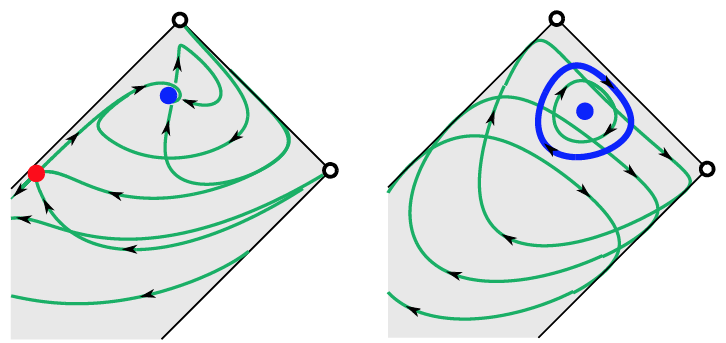
\includegraphics[scale=.8]{./images/bifurcation1.png}
\caption[Scott Hotton.]{A bifurcation from a fixed point to a periodic orbit in an (open) phase portrait in a 2-dimensional activation space.}
\label{F:bifurcation}
\end{figure}
% Replace open phase portrait bifurcation picture with a regular bifurcation picture...

\section{Classifying orbits}

% Consider a revision that does not use invariant sets as a main organizing concept

A phase portrait is a complicated collection of orbits. How can we understand it?  One way is to focus on a few prominent orbits in the phase portrait, and to extrapolate from these to get a sense of how the rest of the system behaves. Oftentimes a system has a few prominent orbits--e.g. certain kinds of stable states that ``pull in'' nearby states--and the rest of the system can be understood relative to those prominent orbits.\footnote{In a more formal presentation, we would focus on  \emph{invariant sets} rather than orbits, which are subsets of a state space with the property that no orbit that enters it will ever leave. Such a set is ``invariant'' in that if a system begins somewhere in an invariant set, it will stay there for all time (Unless some external force pushes it out of the set, but then we no longer have a classical dynamical system.) Notice that a single orbit by itself is an invariant set. Other types of invariant sets contain many orbits.}  For example, in Fig. \ref{F:stateSpaceParts} only 10 orbits are shown (one of which is a single point), but from these 10 orbits we can infer what the other orbits are like. The other orbits are ``between'' these 10. In fact, in this case we can get a pretty good sense of what the system will do just by focusing on the point in the center, and noting that it attracts all other states towards it.
%We have seen that the phase portrait of a dynamical systems sheds some light on how a system behaves. In this section we begin to learn ways to \emph{classify} and talk about these orbits. 

In this section we  introduce some language for classifying orbits and using them to understand the overall behavior of a system. The basic categories we consider are shown in Fig. \ref{F:attractorsRepellers}.

\begin{figure}[h]
\centering
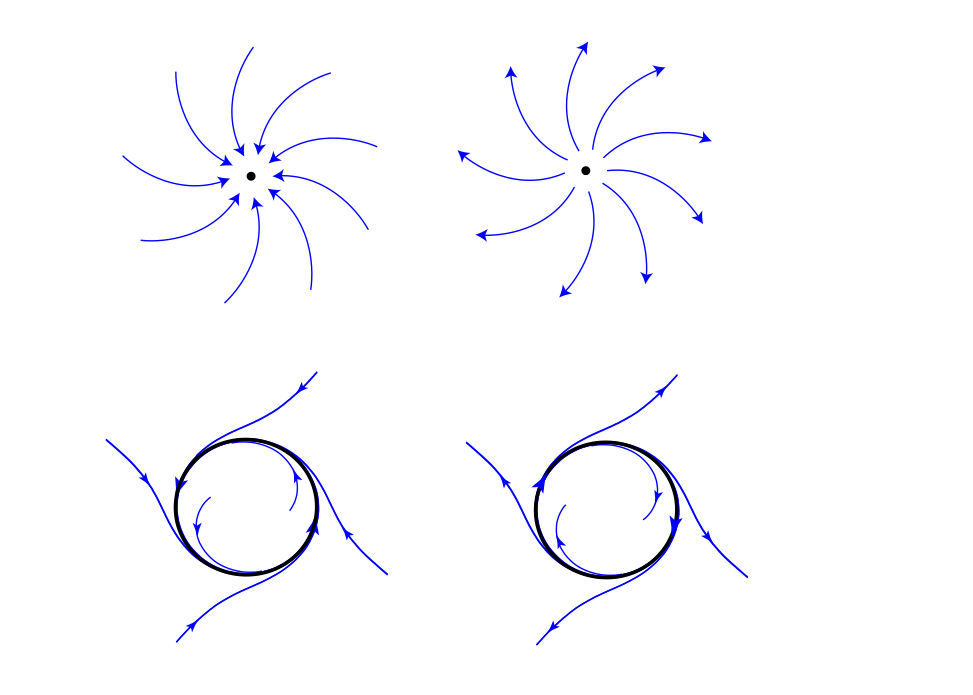
\includegraphics[scale=.5]{./images/AttractorsRepellers.png}
\caption[Pamela Payne.]{An attracting fixed point (upper left), repelling fixed point (upper right), attracting periodic orbit (lower left), and repelling periodic orbit (lower right). Attractors / repellers are shown in black; transient of orbits approaching or leaving attractors and repellers are shown in blue.}
\label{F:attractorsRepellers}
\end{figure}

\subsection{The Shapes of Orbits}

One way to classify orbits is by their shape, or ``topology.''\footnote{The topology of an orbit is its shape, in a special sense. Think of an orbit as a compressible / extendible string. This concept of shape allows arbitrary squashing and pulling of the orbits. Two orbits have the same topology if one can be squashed or squeezed in to the other shape without cutting the strings or gluing them together. In a discrete-time system the topological properties of orbits work differently. Orbits are discrete chains and their topology is defined similarly to how the network diagrams in chapter \extref{ch_intro} were defined.} Some prominent topologies for an orbit are a point, line and a loop. The analogues of these in a discrete time system are a point, a sequence of points, and a cycle of points. 

   The simplest shape for an orbit is a \glossary{fixed point} (also known as an equilibrium), a state that goes to itself under a dynamical system. See the top row of Fig. \ref{F:attractorsRepellers}. This type of orbit is just a single point. When we start a dynamical system  at a fixed point it remains there for all time. Once a system reaches a
fixed point it stays in that state forever. 

Another shape for an orbit is a repeating loop or cycle. See the bottom row of Fig. \ref{F:attractorsRepellers}.\footnote{The Poincar\'{e}-Bendixson theorem tells us there must be at least one fixed point inside the periodic orbits shown on the bottom row of the figure. These fixed points have been omitted for pedagogical purposes.} This kind of orbit periodically visits the same points over and over again. This is a \glossary{periodic orbit}, a set of points that a dynamical system visits repeatedly in the same order. Periodic orbits repeatedly cycle back on themselves. This corresponds to an oscillation in a network, a repeating pattern of firings. For a continuous-time dynamical system, a periodic orbit is loop-shaped (it has the topology of a circle), and its period is the amount of time takes to go around the loop.\footnote{Do not confuse the period of a single periodic  orbit with the number of periodic orbits in the state space. For example, a dynamical system can have one periodic orbit with period 2 and three other periodic orbits with period 5.}
  For a discrete-time system, a periodic orbit is a finite set of $n$ states that the system cycles through (its period is $n$). This is also called an \glossary{n-cycle}. For example, a 2-cycle is a pair of states the system goes back and forth between. A 3-cycle is a set of 3 points that system visits in the same repeating sequence. Similarly for 4,5,100, and arbitrarily large $n$-cycles.

%   Here is the beginning of an orbit for a three node network:
%\begin{small}
%\begin{eqnarray*}
%(-1, 1, 1) \mapsto (-1, -1, 1) \mapsto (1, -1, -1) \mapsto 
%(-1, 1, 1) \mapsto (-1, -1, 1) \mapsto (1, -1, -1) \mapsto \cdots
%\end{eqnarray*}
%\end{small}
%Notice that the first and fourth states are the same. Since dynamical systems 
%are deterministic this implies that the second and fifth states also have to be 
%the same. This applies to the third and sixth states as well. The first, 
%second, and third states are repeated in the fourth, fifth, and sixth states.
%And they have to repeat again in the seventh, eighth, and ninth states. This
%system cycles through these same three states over and over for all of time. 
% n-cycle
% Limit cycle is a special case in 2 dimensions (check notes)
%\footnote{The situation is a little more complicated than this. A periodic orbit for a discrete dynamical system is a finite set of points. A periodic orbit for a continuous system is a closed curve. We often skip over the distinction between discrete and continuous dynamical systems in the main text.}  
% Image of one of these

There are other shapes besides points, lines and loops. Some orbits in higher dimensions are donut shaped ``tori'', for example. Others are even more complex, e.g. fractal shaped.
% Images of fractals etc. More on their significance.

\subsection{Attractors and Repellers}

   Another way we can classify orbits is according to how states near  them behave. Sometimes states near an orbit will tend to  go toward the orbit. It's as though the orbit ``pulls in'' all nearby points. See the left side of Fig. \ref{F:attractorsRepellers}. The fixed point and periodic orbit seem to draw other orbits to towards them. These are \emph{attractors}. More formally, an \glossary{attractor} is an orbit such that all states sufficiently close  to it will stay close to it. If you perturb a system slightly from an attracting state it will tend to go back to that state. Attracting fixe points are also called \emph{stable states} or \emph{stable equilibria}. These are states we are generally more likely to observe a system in. A chair or coin at rest, or a marble at the bottom of a bowl, are at attracting stable states. Move them a little and they will settle right back down. 

 In other cases states near an orbit will tend to go away from the orbit.
It's as though the orbit ``pushes away'' all nearby points. See the right side of Fig. \ref{F:attractorsRepellers}. Once a dynamical system starts running we are unlikely to see it near one of these 
orbits. More formally, a \glossary{repeller} is an orbit such that all states sufficiently close 
to it move away from it.\footnote{Technically these are definitions for 
``attracting sets'' and ``repelling sets''. In order for an attracting set to 
be an attractor or a repelling set to be a repeller the set must satisfy a 
further property known as ``topological transitivity'' which is a concept we
will not go into here. Fixed points and periodic orbits do have this property 
so this definition suffices for them.}  Perturb a system from a repelling state and it will begin to move away from that state. These are also known as ``unstable'' states. A chair or coin resting right on its edge, or a marble balanced precisely at the top of an upside-down bowl, is in a repelling state: move these systems a tiny bit away from their current state and they will go away from that state. Because of this, it is hard to observe systems in repelling states.

When a system has multiple attractors, we can associate each attractor with a \glossary{basin of attraction}, which is the set of all states that tend towards a 
given attractor. This is useful because we can then partition a state space in to basins, one for each attractor. If you start a system off anywhere in the basin of attraction for an attractor eventually it must end up on or very close to that attractor. 
We can think of basins of attraction using a ``hill-and-valley'' metaphor  (see
figure \ref{F:basins}). We can think of the state space of a neural network 
like a wavy surface and we can imagine there is a marble rolling on the surface 
whose position marks the current state of the system. The marble rolls down 
along a path (orbit) in the valley that it starts out in. The attractor in 
this metaphor is the point at the very bottom of the valley that the marble 
comes to rest at and the whole valley is its basin of attraction. The state space in Fig. \ref{F:hopfieldStateSpace} has two attractors with two basins of attraction.
% Talk about basin boundaries, separatrices, etc. 
\begin{figure}[h]
\centering
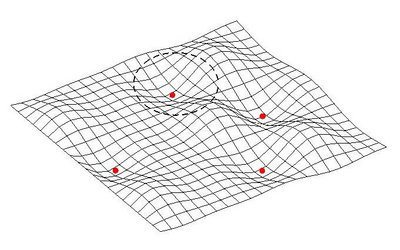
\includegraphics[scale=.5]{./images/BasinAttraction.jpeg}
\caption[From \url{http://www.scholarpedia.org/article/File:Hopfieldattractor.jpg}. Licensed Under CC BY-NC-SA]{Attractors and basins of attraction pictured using a hill and valley 
metaphor.}
\label{F:basins}
\end{figure}

% Also known as association memory / content addressable memories
% Perceptual completion. Picture to illustrate the phenomenon. See unsupervised chapter
As noted above, attractors of recurrent networks can be thought of as memories in some connectionist models. If a network of this kind has 20  attractors, we can think of it as having 20 memories. Recalling a memory corresponds to setting the system in an initial state and letting it settle in to the attractor of whatever basin of attraction it began in. Learning new memories corresponds to modifying the weights of the network to acquire new attractors. A related  example is perceptual completion. Perceptual completion is when you see part 
of a picture and ``fill in'' the rest in your imagination. We can think of 
the state of seeing only part of the picture as being an initial condition in a 
neural network. And we can think of the process of ``filling in'' the rest of 
the picture as the network's dynamical processing that leads to the attractor 
which corresponds to the memory of the whole image. 
% Cues that will trigger a memory or classification. Initial states that end up in the same minimum. Initial configurations of vehicles that will end up spiraling around each other in a particular way.

There are orbits that are neither repellers nor attractors. For example, the central point in Fig. \ref{F:hopfieldStateSpace} is attracting in one direction, and repelling in another.

\subsection{Combining these classifications}

Combining the results of the last two subsections, we can classify the orbits of a dynamical system in terms of the topology of its orbits \emph{together} with whether they are attracting or repelling. This classification is evident in Fig. \ref{F:attractorsRepellers}. Here is the same classification in table form. In the table below, the columns correspond to different topologies or shapes  that an orbit can have. The rows corresponds to the behavior of  states nearby the orbit.
\begin{center}
\begin{tabular}{| l | p{3cm} | p{3cm}|}
\hline
& {\bf Fixed Point} & {\bf Periodic orbit}  \\
\hline
{\bf Attractor} & attracting fixed point & attracting periodic orbit  \\
\hline
{\bf Repeller} &  repelling fixed point & repelling periodic orbit  \\
\hline
\end{tabular}
\end{center}

Recurrent networks displaying all four types of orbit can  be created in Simbrain using the projection plot. However, as noted above, it's easier to find attractors than repellers. Fig. \ref{F:simbrainStateSpace} shows a system with two attracting fixed points on the left, and a system with an attracting periodic orbit on the right. Both are projections of orbits of a 25 dimensional system to 2 dimensions. In both cases the image was generated by repeatedly randomizing network nodes (setting them in an initial condition), running the network, and observing the resulting orbits. About 17 initial conditions were used for the network on the left, and 5 on the right. It is possible that the systems contain more attractors than are shown, but that they were not found after that many attempts. Notice that attractors were found, but not repellers. To find a repeller you have to get lucky and land right on top of it, or find it using mathematical means. This emphasizes the mix of exploratory and more \emph{a priori} or analytic modes of research involved in dynamical systems theory.\footnote{Notice that the orbits are not smooth. This emphasizes that a computer produces a discrete approximation of continuous time processes.} 
% Refer back to discrete time processes

\begin{figure}[h]
\centering
\raisebox{-0.5\height}{\fbox{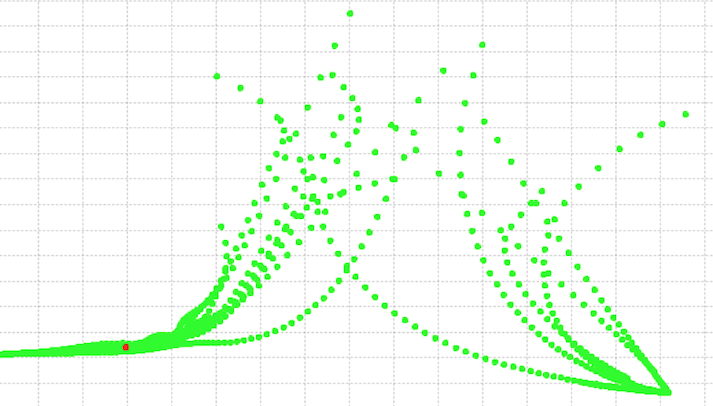
\includegraphics[scale=.45]{./images/projectionFixedPoints.png}}}
\hspace*{.5 in}
\raisebox{-0.5\height}{\fbox{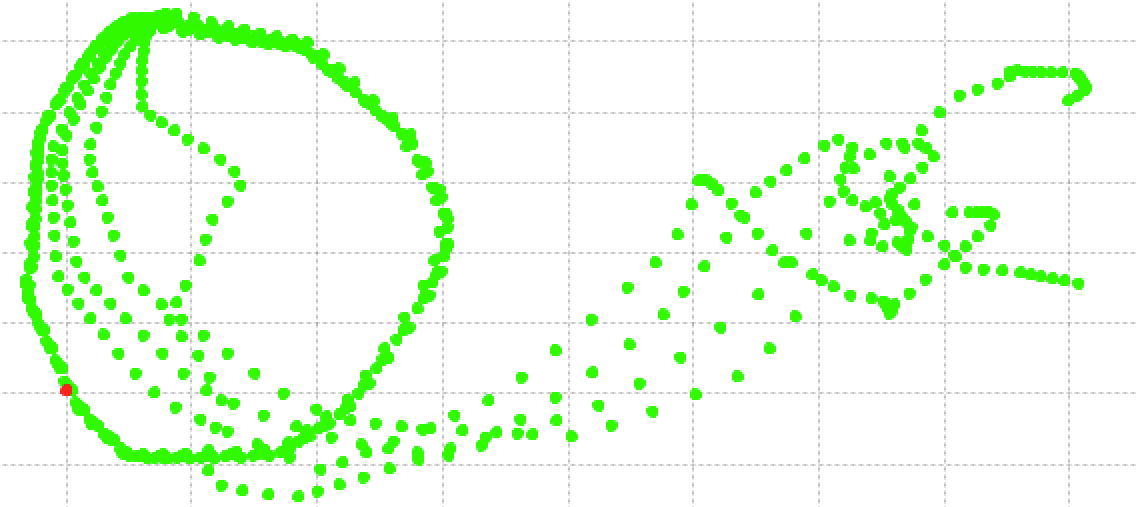
\includegraphics[scale=.35]{./images/projectionPeriodic.png}}}
\caption[Simbrain screenshots.]{Phase portraits generated using Simbrain. A system with two attracting fixed points (Left) and a system with one attracting periodic orbit (Right). Both are projections from a 25 dimensional activation space to 2 dimensions. The red point is the current point in each simulation. }
\label{F:simbrainStateSpace}
\end{figure}
% Keep trying with the image on the right



